\documentclass[12pt]{article}
\usepackage[letterpaper, margin=0.8in]{geometry}
%\usepackage{a4wide}
\usepackage[utf8x]{inputenc}
\usepackage{amsmath, amsthm, amssymb}
\usepackage{times}
\usepackage{verbatim}
\usepackage{graphicx}
\usepackage{amsmath}
\usepackage{slashed}
\usepackage{float}
\usepackage{caption}
\usepackage{enumerate}
\usepackage{bbold}
\usepackage{listings} %\begin{comment}..\end{comment}
\makeatletter
\renewcommand*\env@cases[1][1.2]{%
  \let\@ifnextchar\new@ifnextchar
  \left\lbrace
  \def\arraystretch{#1}%
  \array{@{}l@{\quad}l@{}}%
}
\makeatother



\begin{document}
\title{}
\date{}
\author{Sebastian Merkt}
%\maketitle

\begin{figure}[H]
	\centering
  \includegraphics[scale=0.8]{contour2D.pdf}\\
%	\caption{\textit{Green: } 68\% CL contour for $\bar c_W$ and $\bar c_Z$. \textit{Yellow: } 95\% CL contour for $\bar c_W$ and $\bar c_Z$. \textit{Black: } Minimum value. }
\end{figure}

\begin{figure}[H]
	\centering
  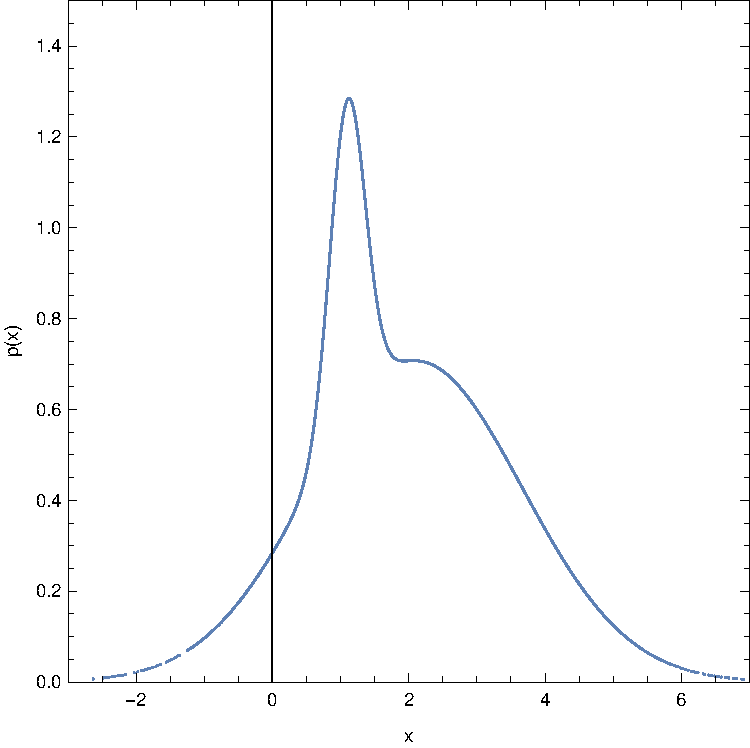
\includegraphics[scale=0.8]{margin.pdf}\\
%	\caption{\textit{Green: } 68\% CL contour for $\bar c_W$ and $\bar c_g$. \textit{Yellow: } 95\% CL contour for $\bar c_W$ and $\bar c_g$. \textit{Black: } Minimum value. }
\end{figure}










\end{document}






